
\chapter{Experimental data on ${IP_3R}$ dynamics (Mak et al.)}

There is an abundance of models for $Ca^{2+}$ signalling, as discussed. In this work we aim to develop an accurate model for $Ca^{2+}$ signalling occurring in the mammalian egg at fertilisation. We are therefore concerned with modelling the $IP_3R$ on the ER accurately. For an oocyte, the only $Ca^{2+}$-releasing channels are the $IP_3R$ as the $RyR$ are not expressed in the ER membrane \cite{dupont}. The open probability of the $IP_3R$ is controlled by several ligands, the most significant of which are $IP_3$ and $Ca^{2+}$. Henceforth, we will refer to the open probability of the $IP_3R$ as $P_O$. $P_O$ is given as follows:
\begin{equation}
    P_O=p_1p_2p_3,\label{openprob}
\end{equation}
where $p_1$ and $p_2$, respectively, represent the probabilities that sites 1 and 2 (for $IP_3$ and $Ca^{2+}$) are activated, and $p_3$ is the probability that $Ca^{2+}$ is not bound to site 3, as in \citeA{atri}. This relatively simple equation presented in \citeA{atri} is shown in equation \eqref{atristeadystate}. Constants were chosen in order to reproduce the steady-state curve for $P_O$, based on data by \citeA{parysetal}. The time constant in equation \eqref{n} for $n$ accounts for the delay between activation and inactivation. A typical timescale {for activation of site 3} used in gating models like those of \citeA{atri} and \citeA{lirinzel} is 1-2 seconds. These can be seen in equations \eqref{origatri1st} and \eqref{lirinzeltwovar1}. This estimate is based on {older} data from \shortciteA{finchetal}, \shortciteA{combettes1994calcium}, \shortciteA{dufour}, and \shortciteA{marchantandtaylor1998}. However, we now have at our disposal experimental data from \citeA{Mak1998} {that accurately capture how the $IP_3R$ dynamics depend on $[Ca^{2+}]$ and $[IP_3]$ during fertilisation}. The newer data confirm the accuracy of this estimate of 1-2 seconds for the measurement of the time dependence but give more details on how the open probability depends on both $Ca^{2+}$ and $IP_3$. To fully understand how the open probability of the $IP_3R$ behaves, it is important to study the steady-state open probability as a function of $IP_3$ and $Ca^{2+}$. For fixed $IP_3$ concentration, the shape of $P_O$ is a bell-shaped function of cytosolic $Ca^{2+}$ concentration. $P_O$ increases at low $Ca^{2+}$, reaches a peak, and then decreases at high $Ca^{2+}$. This can be seen in Figure \ref{foskettfig2}. The precise shape of this curve is dependent upon the $IP_3R$ type and the cell type in some cases. Old data from \shortciteA{kaftan1997} and \shortciteA{hagar1998} suggest a maximum $P_O$ of less than $0.1$. This statistic contradicts more recent studies that estimate to be $P_O$ from $0.3$ to $0.8$ \cite{Mak1998}. The data in \citeA{Mak1998} are single channel data from native membranes as opposed to some artificial system where we cannot say if the exact conditions mimic the cell. This means that we have data which show a very close replicate of how a real egg behaves.

The experimental data provided by \citeA{Mak1998} provide detailed information about the $IP_3R$ gating mechanisms as $Ca^{2+}$ and $IP_3$ bind to the $IP_3R$, activating $Ca^{2+}$ release from the ER. These dynamics drive complicated cytoplasmic $Ca^{2+}$ signals, including temporal oscillations and propagating waves. It is evident that both positive and negative feedback of cytosolic $Ca^{2+}$ controls the $IP_3$-mediated $Ca^{2+}$ release. The experiment was carried out under rigorously defined conditions using patch clamp of the $IP_3R$ in the ER membrane of isolated Xenopus Laevis oocyte nuclei. The results provided detailed information about how the $IP_3R$ works and the dependence on cytosolic $Ca^{2+}$ and $IP_3$. In Figure \ref{foskettfig1a} typical traces of single-channel current for different levels of $Ca^{2+}$ are shown. When cytosolic $Ca^{2+}$ concentration is at steady-state ($0.01-0.1 \mu M$), $P_O$ was low, and some short open intervals of $\tau_O<3 ms$ are observed. These open intervals were interlaced with much longer closed intervals of approximately $\tau_C=100 ms$, as seen in Figure \ref{foskettfig1b}. As the $Ca^{2+}$ level rose from $0.1 \mu M$ to $1\mu M$, $P_O$ drastically increases up to $0.8$, with $\tau_O$ increasing to around $10ms$ and $\tau_C$ decreasing to around $2ms$. Figure \ref{foskettfig1b} from \citeA{Mak1998} shows the mean time of closed-channel ($\tau_C$) and open-channel ($\tau_O$), as a function of the cytosolic $Ca^{2+}$ level.

\begin{figure}[h!!!t!!!b!!!p]
  \centering
  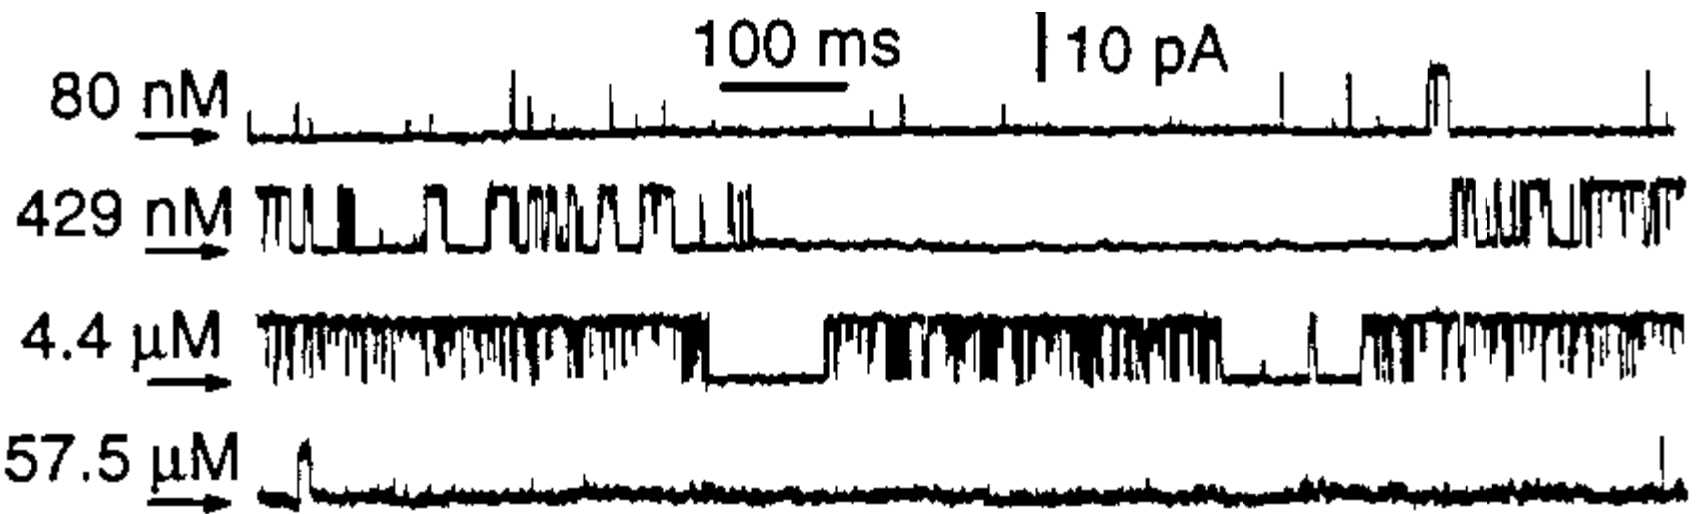
\includegraphics[width=1\linewidth]{Chapters/3_IP3R_dynamics/extras/fig1afoskett.PNG}
  \caption{Closed-channel current levels in each trace recorded at various levels of $Ca^{2+}$: $80 nM$, $429 nM$, $4.4 \mu M$ and $57.5 \mu M$, in the presence of $10 \mu M$ of $IP_3$. Source: \citeA{Mak1998}. }\label{foskettfig1a}
\end{figure}
\begin{figure}[h!!!t!!!b!!!p]
  \centering
  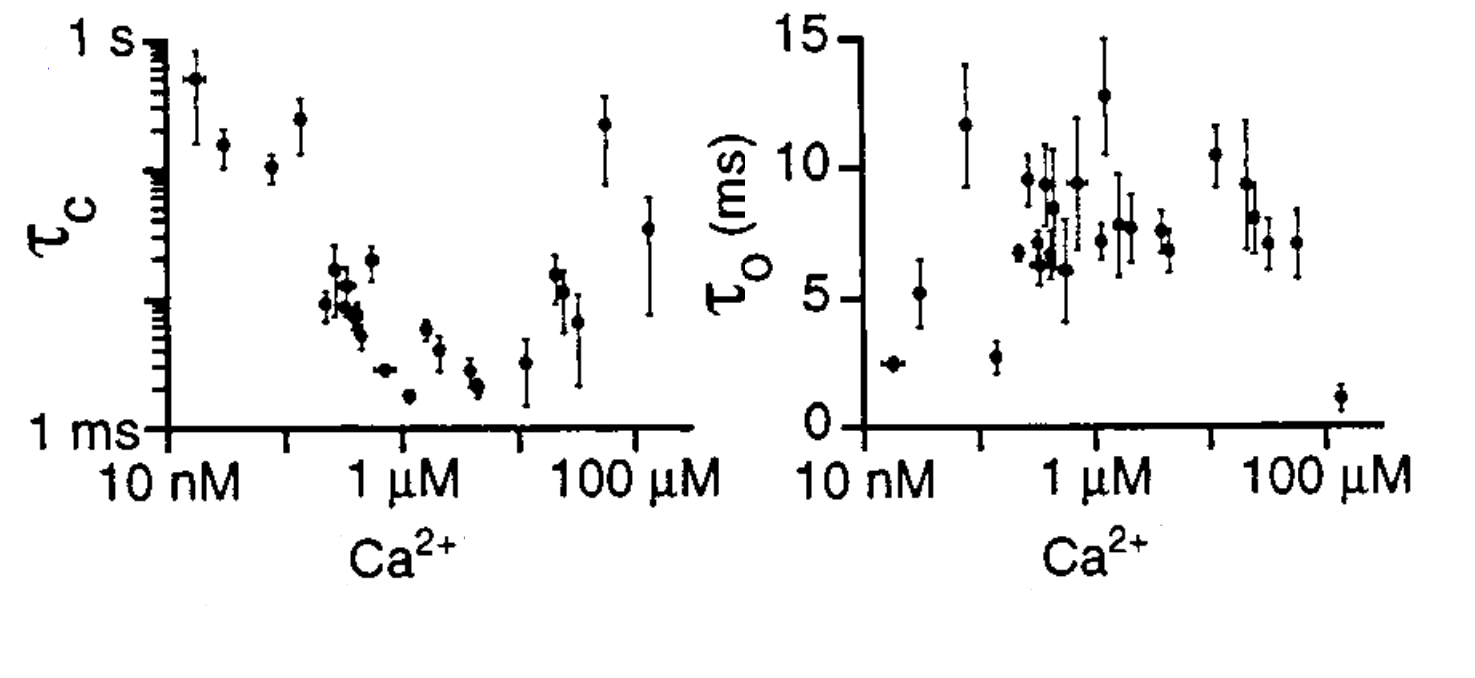
\includegraphics[width=1\linewidth]{Chapters/3_IP3R_dynamics/extras/fig1bfoskett.PNG}
  \caption{Mean time of closed-channel ($\tau_C$) and open-channel ($\tau_O$), in the presence of $10 \mu M$ of $IP_3$, as a function of the cytosolic $Ca^{2+}$ level. Source: \citeA{Mak1998}. }\label{foskettfig1b}
\end{figure}
\subsubsection*{${\mathbf{Ca^{2+}}}$ dependence of the gating of the $\mathbf{IP_3R}$}

In the experiment, \citeA{Mak1998} expected to observe a narrow bell-shaped curve for $P_O$ when the cytosolic $Ca^{2+}$ is approximately $300nM-1 \mu M$ \shortcite{Bezprozvannyehrlich, Bezprovannywatras, Stehno-Bittel1995,Iino}. However, the results clearly showed that the open probability of the gate remained elevated at approximately $0.8$ with saturating levels of $IP_3$ ($10\mu M$) applied to the cytosol to fully stimulate at various levels of $Ca^{2+}$ concentrations. This can be seen in Figure \ref{foskettfig2}. It was only upon increasing the $Ca^{2+}$ levels above $20\mu M$ that the open probability, $P_O$, drastically started to decrease. This is due to the two distinct types of functional $Ca^{2+}$ binding sites, activating and inhibitory ones.

\citeA{Mak1998} derived an equation to accurately model their experimental data for the open probability of the $IP_3R$. This equation for $P_O$ is considered a breakthrough in the modelling of the $IP_3R$ dynamics. It is formatted slightly differently to the open probability in other models, as follows. 
\begin{equation}
    P_O=P_{max}{\left(\frac{1}{1+\left(\frac{K_{act}}{c}\right)^{H_{act}}}\right)}{\left(\frac{1}{1+\left(\frac{c}{K_{inh}}\right)^{H_{inh}}}\right)},\label{foskett}
\end{equation}
where
\begin{equation}
    K_{inh}=K_{\infty}\left(\frac{1}{1+\left(\frac{K_{IP_3}}{p}\right)^{H_{IP_3}}}\right).\label{kinheqn}
\end{equation}
{This equation is phenomenological, based on experimental data obtained for the single channel $IP_3R$. }The first parenthesis in equation \eqref{foskett} models $Ca^{2+}$ binding to the activation site. The second parenthesis models $Ca^{2+}$ binding to the inhibitory site. $K_{inh}$ depends on $IP_3$ binding to its activation site. Recall that previous models, \eqref{origatri1st}-\eqref{origatri2nd} and \eqref{lirinzeltwovar1}-\eqref{lirinzeltwovar2}, had these terms for the three sites as three separate parentheses.

Equation (\ref{foskett}) is a `biphasic Hill equation', as referred to in \citeA{Mak1998}. The shape of this as a graph has $P_O$ increasing, reaching a peak, and then decreasing. This can be seen fitting to the data in Figure \ref{foskettfig2}.  Parameter values are given in Table \ref{foskettparam}. The maximum probability of the $IP_3R$ channel being open, $P_{max}$, is given as {$0.81$}. This was chosen based on the experimental data where $0.81$ was shown to be the maximum value, as seen in Figure \ref{foskettfig2}. This equation models the two distinct types of binding sites for $Ca^{2+}$ - the activation and inhibitory sites. The activation and inhibition of the $IP_3R$ by $Ca^{2+}$ are very cooperative processes and this is represented by the Hill coefficients chosen, $H_{act}=1.9 \pm 0.3$ and $H_{inh}=3.9 \pm 0.7$. These also suggest that it is necessary for $Ca^{2+}$ to bind to two of four monomers to open the $IP_3R$ channel in the presence of $IP_3$, and for $Ca^{2+}$ to bind to all four monomers to prevent opening of the channel \cite{Mak1998}.

Lowering the $IP_3$ concentration did not affect $Ca^{2+}$ activation parameters or the Hill coefficient for the term representing $Ca^{2+}$ binding to the inhibitory site, $H_{inh}$. This did however decrease the half-maximal inhibitory $Ca^{2+}$, $K_{inh}$. Also observed was a functional half-maximal activating $IP_3$ concentration, $K_{IP_3}$, at $50nM$ and a corresponding Hill coefficient, $H_{IP_3}$, at 4 for $IP_3$. From these results it is apparent that $Ca^{2+}$ is a receptor agonist{, as it stimulates the opening of the channel with sufficient $IP_3$ present} \cite{Berridge2000}. The evidence suggests that the sole function of $IP_3$ is to relieve $Ca^{2+}$ inhibition. The results of the experiments are shown in Figure \ref{foskettfig2}. 

\subsubsection*{Dependence of $\mathbf{P_O}$ on $\mathbf{IP_3}$}
The results of the experimental data in \citeA{Mak1998} suggest that the open probability of the $IP_3R$ is relatively insensitive to $Ca^{2+}$ until it reaches a quite high concentration. This insensitivity is in contrast to previous models which have assumed a higher affinity of $Ca^{2+}$ binding to the inhibitory site. This was, therefore, further investigated by \citeA{Mak1998} but there was evidently no change in $Ca^{2+}$ dependence with ranging concentration of $IP_3$. This is proof that the $IP_3R$ has a low-affinity $IP_3$ binding site with binding coefficients  greater than $0.1 \mu M$. There are many biochemical data that match this \shortcite{mauger,taylortraynor,taylorrichardson,josephs}. As $IP_3$ was lowered to less than $0.1\mu M$, the channel became more sensitive to $Ca^{2+}$ inhibition, as seen in Figure \ref{foskettfig2}. For example, at $0.033 \mu M$ of $IP_3$, $K_{inh}$ was brought all the way down to $9.5 \mu M$, though constants for $Ca^{2+}$ binding to the activation site were unaffected. In comparison, at an $IP_3$ concentration of $10\mu M$, $K_{inh}$ lies at $54 \mu M$. When much lower levels of $IP_3$ were applied, there was a significant reduction in both the maximum open probability, $P_{max}$ and the range of $Ca^{2+}$ for which the channel was active. With $K_{inh}$ as the only $IP_3$-sensitive parameter, equation \eqref{kinheqn}, accurately fits with experimental data carried out for a wide range of $IP_3$ concentrations. \citeA{Mak1998} concluded that the effect of $IP_3$ binding is not to enable $Ca^{2+}$ binding to the activation site, but to ameliorate $Ca^{2+}$ binding to the inhibitory site. Previously, it was thought that the effect of the binding was to enable activation of the $IP_3R$ by $Ca^{2+}$ \shortcite{mauger, taylorrichardson, taylortraynor, josephs}, but the data from \citeA{Mak1998} suggest otherwise. The dependence of $K_{inh}$ on the $IP_3$ concentration is described with the Hill equation \eqref{foskettkinhip3}. Figure \ref{foskettcurve} shows $P_O$ against $Ca^{2+}$ concentration with various chosen levels of $IP_3$ (and the respective values for $K_{inh}$ according to equation \eqref{foskett}). Figure \ref{foskettfig2} shows how the derived equation for $P_O$ fits the data well. 
\begin{figure}[h!!!t!!!b!!!p]
  \centering
  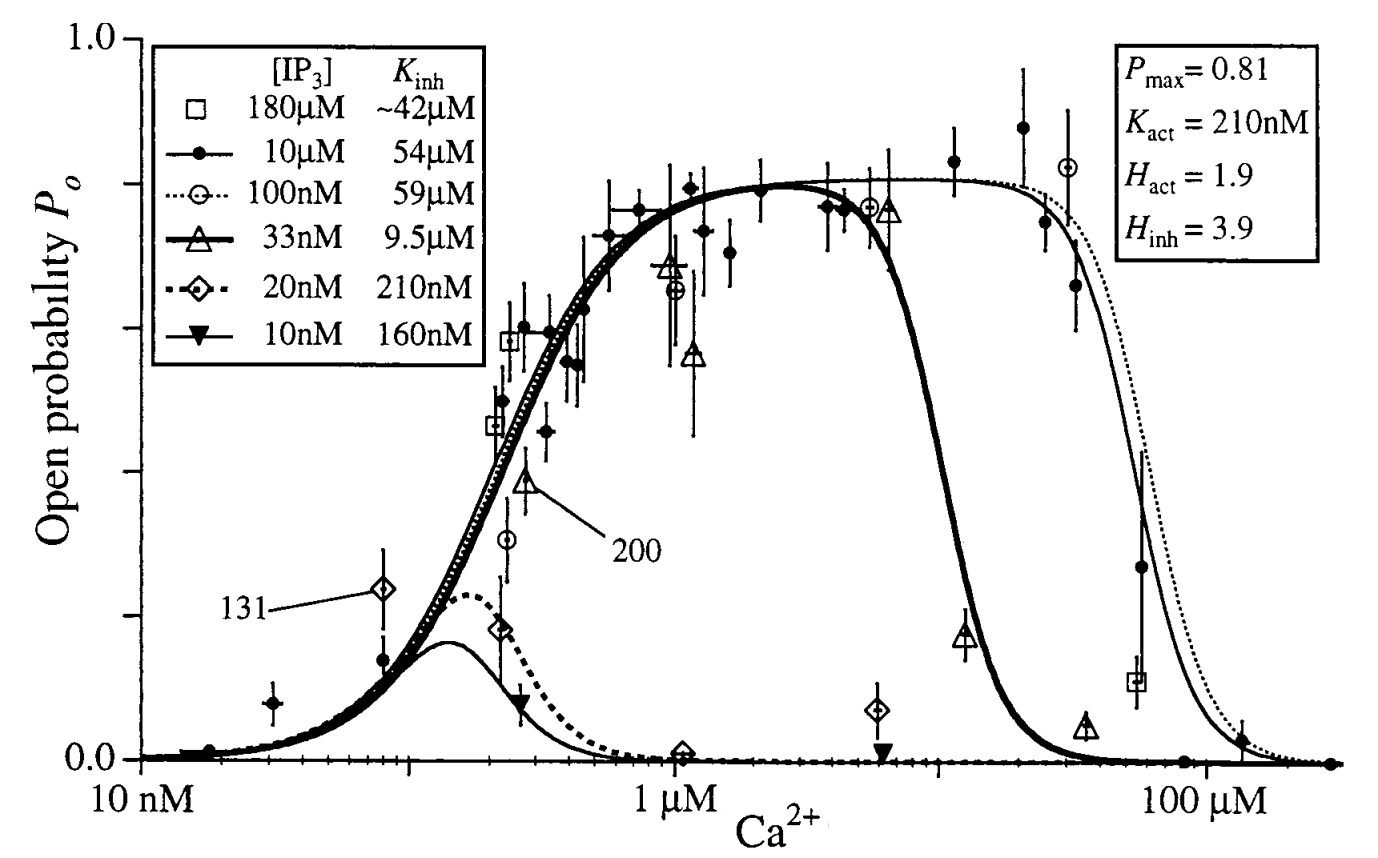
\includegraphics[width=1\linewidth]{Chapters/3_IP3R_dynamics/extras/fig2foskett.png}
  \caption{$P_O$ as $Ca^{2+}$ varies, at different levels of $IP_3$. We can see how the equation \eqref{foskett} fits the data well. Source: \citeA{Mak1998}. }\label{foskettfig2}
\end{figure}

\begin{figure}[h!!!t!!!b!!!p]
  \centering
  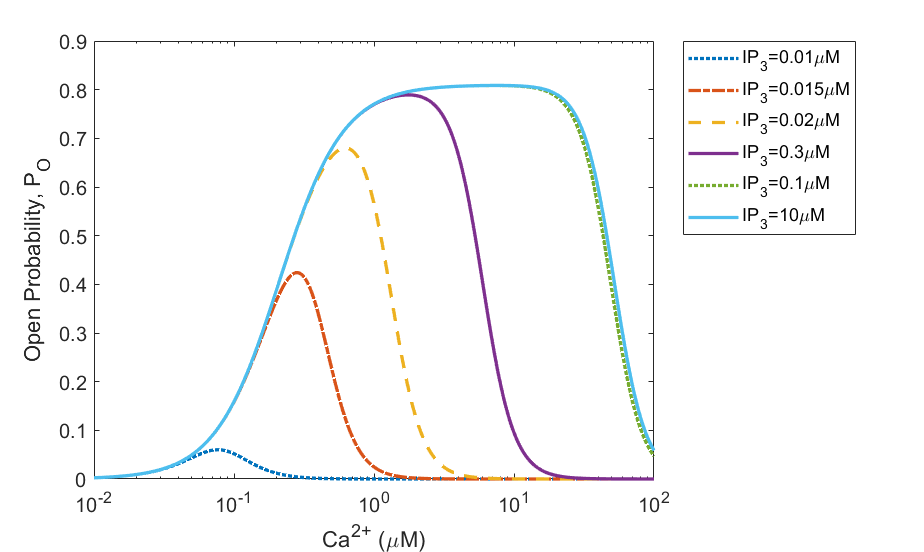
\includegraphics[width=1\linewidth]{Chapters/3_IP3R_dynamics/extras/fosketthillfunction.png}
  \caption{The open probability \eqref{foskett} of $IP_3$, $P_O$, as a function of the cytosolic $Ca^{2+}$ for a series of $IP_3$ values. Parameters used are shown in Table \ref{foskettparam}. \textit{Software:} MATLAB.}\label{foskettcurve}
\end{figure}

As discussed, the only $IP_3$-concentration-sensitive parameter here is $K_{inh}$. This parameter was shown to decrease with decreasing $IP_3$. The equation for $K_{inh}$ indicates that the $IP_3R$ has a single class of functional $IP_3$ binding sites. Figure \ref{kinhvsp} demonstrates how $K_{inh}$ varies with increasing $IP_3$. Table \ref{foskettkinhip3} presents a range of numerical values computed for $K_{inh}$ at fixed $IP_3$. Also shown in Figure \ref{kinhvsp} are examples of the bell shape attained with normalised $P_O$ vs. $Ca^{2+}$. These were computed from equation \eqref{foskett} with three different values for $IP_3$ chosen.

\begin{figure}[!htb]
\minipage{0.5\textwidth}
  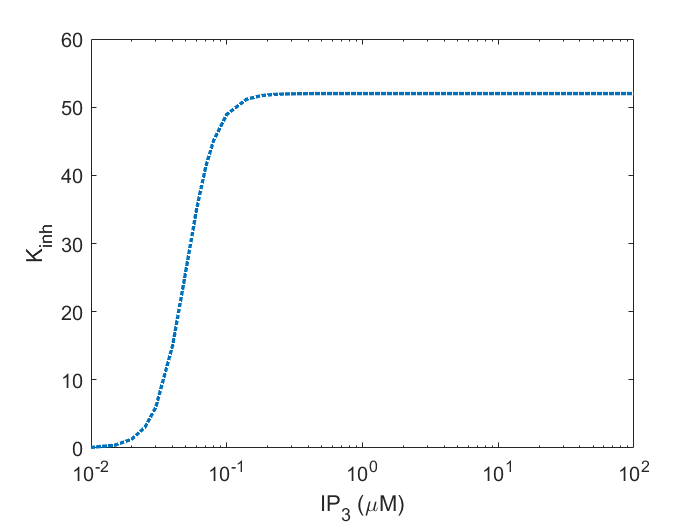
\includegraphics[width=\linewidth]{Chapters/3_IP3R_dynamics/extras/kinhvsp.png}
\endminipage\hfill
\minipage{0.5\textwidth}
  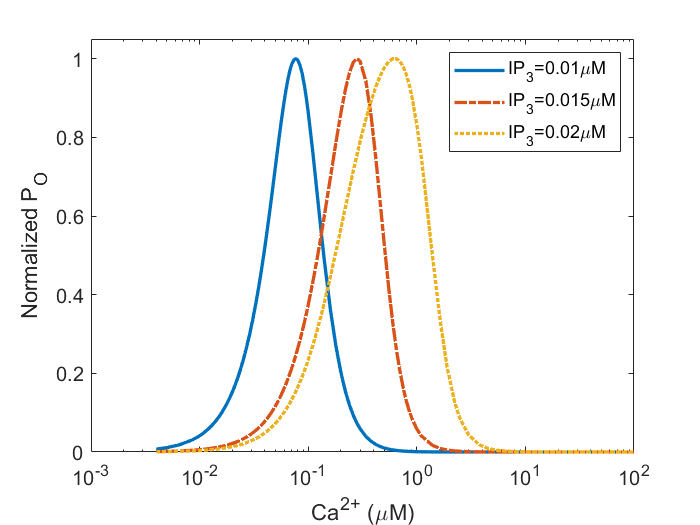
\includegraphics[width=\linewidth]{Chapters/3_IP3R_dynamics/extras/fig3bfoskettmatlab.png}
\endminipage\hfill
\caption{(Left) $K_{inh}$ for increasing $IP_3$ concentration ($\mu M$). (Right) Bell-shaped normalised $P_O$ vs. cytosolic $Ca^{2+}$ concentration, from equation \eqref{foskett}. The blue solid line is for $IP_3=0.01 \mu M$, with a maximum point of $0.09$. The red dashed line is for $IP_3=0.015\mu M$, with a maximum point of $0.49$. Finally, the yellow dotted line is for $IP_3=0.02$, with a maximum at $0.71$ \cite{Mak1998}. \textit{Software:} MATLAB.}\label{kinhvsp}
\end{figure}

\begin{table}[h!!!t!!!b!!!p]
\begin{center}
\begin{tabular}{ c c }
$IP_3$ ($\mu M$) & $K_{inh}$ ($\mu M$)\\
\hline
$180$ & $\sim 42$\\
\hline
$10$ & $54$\\
\hline
$0.1$ & $59$\\
\hline
$0.033$ & $9.5$\\
\hline
$0.02$ & $0.21$\\
\hline
$0.01$ & $0.16$\\
\end{tabular}
\end{center}
\caption{$K_{inh}$ ($\mu M$) for given $IP_3$ concentrations ($\mu M$) from equation \eqref{kinheqn}. See also Figure \ref{kinhvsp}.}\label{foskettkinhip3}
\end{table}

The maximum inhibitory $Ca^{2+}$ binding coefficient is given by $K_{\infty}$. This parameter was assigned a value of $52 \pm 4 \mu M$ at a saturating $IP_3$ concentration. The value of $K_{IP_3}$ derived is a close match to the dissociation constant in $IP_3$ binding assays as well as the necessary $IP_3$ concentration needed to stimulate $Ca^{2+}$ release \shortcite{mauger, taylortraynor, josephs, meyer}. The large Hill coefficient of $4 \pm 0.5$ for $H_{IP_3}$ in equation \eqref{kinheqn} is due to $IP_3$ activation of the $IP_3R$ being a very cooperative process \shortcite{meyer, finchetal, carterodgen, dufour}. This means that we require $IP_3$ binding to all four monomers to open the gate of the channel through relieving $Ca^{2+}$ inhibition. Figure \ref{fig3c} portrays the theoretical $P_O$ equation, \eqref{foskett}, for different levels of $Ca^{2+}$ as $IP_3$ is increased.

\begin{figure}[h!!!t!!!b!!!p]
  \centering
  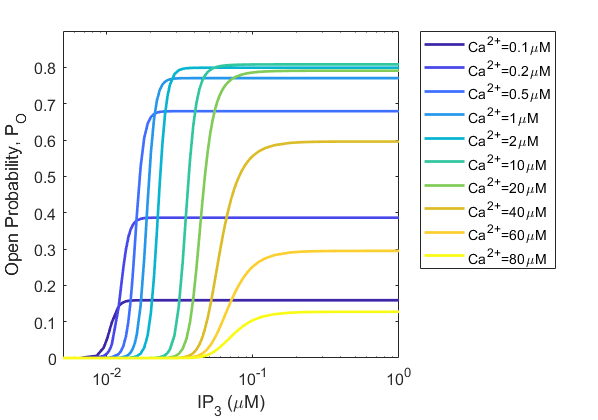
\includegraphics[width=0.8\linewidth]{Chapters/3_IP3R_dynamics/extras/fig3cfoskettmatlab.png}
  \caption{{Replication of Figure 3c in \citeA{Mak1998}. It displays $P_O$ from equation \eqref{foskett} vs. cytosolic $IP_3$ concentrations, at various levels of cytosolic $Ca^{2+}$ concentrations. \textit{Software:} MATLAB.} }\label{fig3c}
\end{figure}

As seen in Figure \ref{foskettcurve}, the data from \citeA{Mak1998} clearly show a bell-shaped relationship between $P_O$ and $Ca^{2+}$ with a sharp peak for $Ca^{2+}<1\mu M$ at low ($<0.02\mu M$) $IP_3$. The experiments imply that although cytosolic $Ca^{2+}$ (at low concentrations) and $IP_3$ both activate the $IP_3R$ channel, they do so in different ways. Like a conventional agonist, $Ca^{2+}$ binding at low levels directly activates the channel. When the $IP_3$ concentration is low, $Ca^{2+}$ is more likely to bind to the inhibitory site because of its higher affinity ($K_{inh}<K_{act}$). When the $IP_3$ concentration is higher, this is reversed. A visual representation of this is shown in Figure \ref{foskett3d1} \cite{Mak1998}.

\begin{figure}[!htbp]
\centering
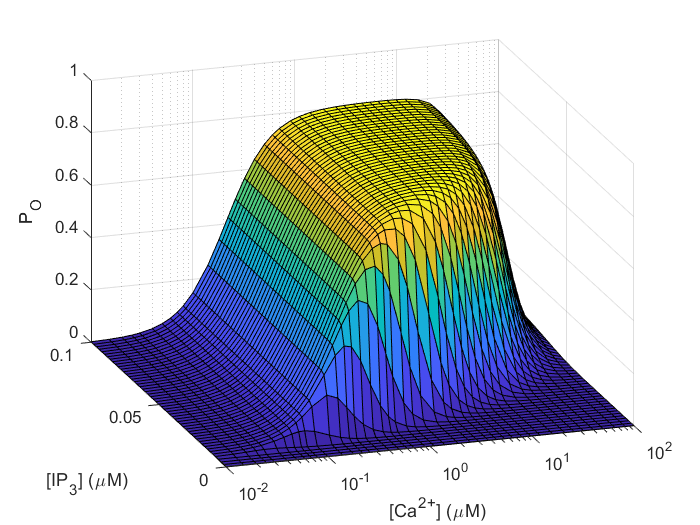
\includegraphics[width=0.7\linewidth]{Chapters/3_IP3R_dynamics/extras/foskett3D2.png}
\caption{$P_O$ vs. $IP_3$ vs. $Ca^{2+}$. $P_O$ works at low, `activating', levels of $Ca^{2+}$. $P_O$ varies with changing $IP_3$ concentration. We can also see the effects on $P_O$ at high, `inhibitory', levels of $Ca^{2+}$. Parameter values used are shown in Table \ref{foskettparam} \cite{Mak1998}. \textit{Software:} MATLAB.}\label{foskett3d1}
\end{figure}

The experimental data and corresponding equation fitted to them in \citeA{Mak1998}, \eqref{foskett}, is the most up to date equation for the open probability of the $IP_3R$, capturing that $IP_3$ mediates its effects by modulating the affinity of $Ca^{2+}$ inhibitory sites \cite{Mak1998}. It is thus, a vital component of a $Ca^{2+}$ signalling model at fertilisation. We will therefore endeavor to develop a model with this $P_O$, using the {structure of the} Atri model. To achieve this we must study carefully the Atri model and see how we can replace appropriately the components modelling $Ca^{2+}$ binding to its activation site, $Ca^{2+}$ binding to its inhibitory site, and $IP_3$ binding to its activation site.

Before doing so, we study the model by \citeA{swedish} where they have incorporated the open probability curve by \citeA{Mak1998} into a $Ca^{2+}$ signalling model. We present a summary of this model in the following chapter.